% ****** Start of file apssamp.tex ******
%
%   This file is part of the APS files in the REVTeX 4.2 distribution.
%   Version 4.2a of REVTeX, December 2014
%
%   Copyright (c) 2014 The American Physical Society.
%
%   See the REVTeX 4 README file for restrictions and more information.
%
% TeX'ing this file requires that you have AMS-LaTeX 2.0 installed
% as well as the rest of the prerequisites for REVTeX 4.2
%
% See the REVTeX 4 README file
% It also requires running BibTeX. The commands are as follows:
%
%  1)  latex apssamp.tex
%  2)  bibtex apssamp
%  3)  latex apssamp.tex
%  4)  latex apssamp.tex
%
\documentclass[%
 reprint,
%superscriptaddress,
%groupedaddress,
%unsortedaddress,
%runinaddress,
%frontmatterverbose, 
%preprint,
%preprintnumbers,
%nofootinbib,
%nobibnotes,
%bibnotes,
 amsmath,amssymb,
 aps,
%pra,
%prb,
%rmp,
%prstab,
%prstper,
%floatfix,
]{revtex4-2}
\usepackage[table,xcdraw]{xcolor}
\usepackage{graphicx}% Include figure files
\usepackage{dcolumn}% Align table columns on decimal point
\usepackage{bm}% bold math
%\usepackage{hyperref}% add hypertext capabilities
%\usepackage[mathlines]{lineno}% Enable numbering of text and display math
%\linenumbers\relax % Commence numbering lines

%\usepackage[showframe,%Uncomment any one of the following lines to test 
%%scale=0.7, marginratio={1:1, 2:3}, ignoreall,% default settings
%%text={7in,10in},centering,
%%margin=1.5in,
%%total={6.5in,8.75in}, top=1.2in, left=0.9in, includefoot,
%%height=10in,a5paper,hmargin={3cm,0.8in},
%]{geometry}

\begin{document}

\preprint{APS/123-QED}

\title{Reading project: Fundamentals of Quantum Mechanics }% Force line breaks with \\
\thanks{Primarily from Cohen Tannoudje: Quantum Mechanics}%

\author{Rishi Paresh Joshi }
\altaffiliation[At]{School of Physical Sciences, NISER}
\affiliation{Under Dr.Kush Saha, School of Physical Sciences, NISER}%
 
 %Lines beak automatically or can be forced with \\


\date{\today}% It is always \today, today,
             %  but any date may be explicitly specified

\begin{abstract}
Certain Fundamental ideas of quantum mechanics are introduced and discussed, in a qualitative and intuitive manner.How the quantum description of physical systems differs radically from the one given by classical mechanics (although the latter constitutes, in numerous cases, an excellent approximation) is made clear. In this project we have restricted the discussion of physical systems composed of only one particle. The description of these systems at a given time is, in classical mechanics, founded on the specification of six parameters, which are the components of the position $\mathbf{r}(t)$ and the velocity $\mathbf{v}(t)$ of the particle. All the dynamical variables (energy, linear momentum, angular momentum) are determined by the specification of $\mathbf{r}(t)$ and $\mathbf{v}(t)$. Newton's laws enable us to calculate $\mathbf{r}(t)$ through the solution of second-order differential equations with respect to time. Consequently, they fix the values of $\mathbf{r}(t)$ and $\mathbf{v}(t)$ for any time $t$ when they are known for the initial time.

Quantum mechanics uses a more complicated description of phenomena. The dynamic state of a particle, at a given time, is characterized by a wave function. It no longer depends on only six parameters, but on an infinite number [the values of $\psi(\mathbf{r}, t)$ at all points $\mathbf{r}$ of space]. Moreover, the predictions of the measurement results are now only probabilistic (they yield only the probability of obtaining a given result in the measurement of a dynamical variable). The wave function is a solution of the Schrödinger equation, which enables us to calculate $\psi(\mathbf{r}, t)$ from $\psi(\mathbf{r}, 0)$. This equation implies a principle of superposition which leads to wave effects.

This upheaval in our conception of mechanics was imposed by experiment. The structure and behavior of matter on an atomic level are incomprehensible in the framework of classical mechanics. The theory has thereby lost some of its simplicity, but it has gained a great deal of unity, since matter and radiation are described in terms of the same general scheme (wave-particle duality). The fact is that this general scheme; although it runs counter to our ideas and habits drawn from the study of the macroscopic domain, is perfectly coherent. No one has ever succeeded in imagining an experiment which could violate the uncertainty principle. In general, no observation has, to date, contradicted the fundamental principles of quantum mechanics. Nevertheless, at present, there is no global theory of relativistic and quantum phenomena, and nothing, of course, prevents the possibility of a new upheaval.

\begin{description}
\item[Glossary]
$E$-Photon energy
$p$-Momentum of the particle
$\overrightarrow{k}$-Wave vector
$\omega$-angular velocity
$\nu$-frequency
\end{description}
\end{abstract}

%\keywords{Suggested keywords}%Use showkeys class option if keyword
                              %display desired
\maketitle

%\tableofcontents

\section{\label{sec:level1}Introduction\protect\\History}
  Newtonian mechanics explained the motion of material bodies. The theory of electromagnetic radiation due to the introduction of Maxwell's equations produced a uniform interpretation of a set of phenomena that had been previously considered in different domains: electricity, magnetism, and optics. The electromagnetic theory of radiation was confirmed experimentally by discovering Hertzian waves. Finally, the interaction between radiation and matter was explained by Lorentz force. The charge was considered as a property of matter. 

Phenomena occurring on a very small scale(atomic or sub-atomic) cannot be explained outside the framework of quantum physics. Even when considering macroscopic phenomena, a complete scientific description is given by quantum mechanics. Quantum mechanics treated particles and radiations on the same footing.
\section{Basic Outline}
Basic quantum ideas covered:
\begin{enumerate}
\item Wave-particle duality: Further extended into material particles 
\item Wave functions Schrodinger equation: Characteristics of wave packets 
\item Heisenberg uncertainty relations 
\end{enumerate}
\subsection{Wave particle duality}
    \subsubsection{Light quanta and Planck-Einstein relation:}
        \begin{enumerate}
            \item Newton considered light as a beam of particles. 
            \item The wave nature of light was shown by phenomena of interference and diffraction  
            \item Black body radiation showed that the only possible energies we get are $n\hbar\omega$; light consists of a beam of photons, which was proved by the Compton effect. 
           \item Interaction of an electromagnetic wave with matter occurs using elementary indivisible processes in which radiation appears to be composed of particles called photons. Particle parameters($E$  and $p$) are linked to wave parameters($\omega$ and $\overrightarrow{k}$).
                   \end{enumerate}
    \begin{equation}
                E=\hbar\omega=h\nu
    \end{equation}
    \begin{equation}
        \mid \overrightarrow{k} \mid=\frac{2\pi}{\lambda} \
    \end{equation}
    \begin{equation}
        p=\hbar\overrightarrow{k}
    \end{equation}
    
\subsubsection{Analysis of Young's double slit experiment:}  
    \texttt{What happens when the source emits photons practically one by one?}\\
\paragraph{Neither predictions of wave theory nor particle theory are verified. 
Results seen are (Refer to Fig\ref{Single photon Young's double slit})}
\begin{enumerate}
\item When the time of exposure is increased, fringes are formed, so the particle interpretation must be rejected.
\item When the time of exposure is less, fringes are not formed, and intensity is localized.
\end{enumerate}
\begin{figure}[h!]
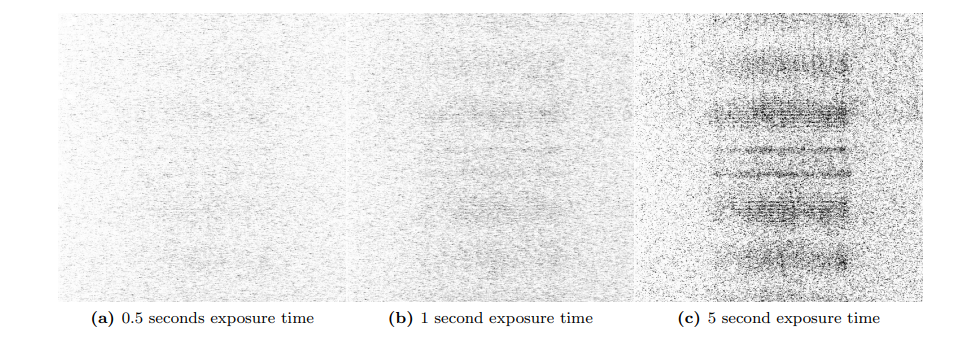
\includegraphics[scale=0.4]
{Double Slit experiment.png}% Here is how to import EPS art
\caption{\label{Single photon Young's double slit} Images of double slit output taken using attenuation of 0.8 × 10$^-^{5}$. The gain was at 255, and each image is contrast adjusted and brightness inverted. From left to right, exposure times were 0.5 seconds, 1 second, and 5 seconds. These images show how the fringe pattern is built over time as more photons are detected. At a 0.5-second exposure time, the detections are largely scattered, but the structure is seen to take shape at 1 second, and the fringe structure seen in the figure is reproduced using a 5-second exposure time.}
\end{figure}
\texttt{Also, the queison arises why the presence of other slits being closed or open affects the final pattern.}\\
To answer this, a new theory was developed, called the Quantumarenification of light. Characteristics of the new quantum domain are that when one measures a microscopic system, it fundamentally disturbs it. Consider placing a detector to detect the number of photons. It will block the light, and thus the pattern will be changed. Therefore, it is impossible to observe the same interference pattern and to know at the same time through which slit each photon has passed.
These things can be summarised into:
\begin{enumerate}
\item Photon doesn't have a fixed trajectory(because it creates an interference pattern over some time).
\item Initial conditions do not predict where the photon strikes.(Only probability of the photon striking can be thought of $\displaystyle \propto I(x)\displaystyle \propto E(x)^2$)
\end{enumerate}
\paragraph{This can be summarised as the Quantum unification of light.}
\begin{enumerate}
\item Particle and wave aspects of light are inseparable. Waves allow us to calculate the probability of manifestation of a particle.
\item $E(x,t)$ is the probability amplitude at time t of photons.
$\displaystyle P(x,t)\displaystyle \propto \mid E(x,t)\mid^2$
\end{enumerate}
\subsubsection{Principle of spectral decomposition} 
Consider a sufficiently intense beam of light traveling in the positive z direction.
\begin{equation}
    E(\overrightarrow{r},t)=E_0e^{ikz-\omega t}\hat{e_p}
    \end{equation}
 It passes through the analyzer and gets polarised in the x-axis direction as shown in the figure.
\begin{figure}[h!]
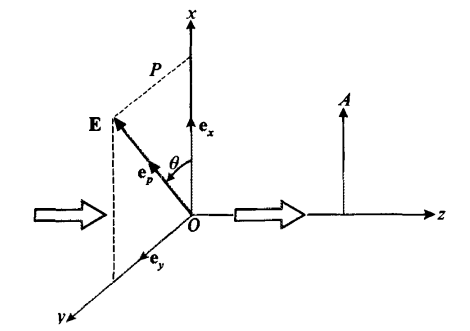
\includegraphics[scale=0.5]{Spectral decomposition.png}
\caption{\label{Spectral decomposition.png} 
 $\theta$ is the angle between the electric field transmitted by P and the x-axis. The electric field of the wave transmitted through A is parallel to the x-axis.}
 \end{figure}
 \\
 \texttt{What will happen when Intensity is low for the photons to reach the analyzer one by one? (We then place a photon detector behind this analyzer.)}\\
 The following are the aspects of the system.
 \begin{enumerate}
\item The detector never registers a fraction of a photon. 
\item From the previous section we know that we cannot predict with certainty whether a given incident photon will pass or be absorbed. We can only know the corresponding probabilities. 
\item If we send out a large number of photons one after the other, the result will correspond to the classical law, in the sense that about an N$Cos^2\theta$ will be detected after the analyzer. 
\end{enumerate}
We shall retain the following ideas from this description 
\begin{enumerate}
 \item The measurement device (the analyzer, in this case) can give only specific privileged results, which we shall call eigen or proper results. In the above experiment, there are only two possible results: the photon crosses the analyzer, or it is stopped.
 \item To each of these eigen results corresponds an eigenstate. Here, the two eigenstates are characterized by:
 $\hat{e_p}=\hat{e_x}$ or $\hat{e_p}=\hat{e_y}$
\item When the state before the measurement is arbitrary, only the probabilities of obtaining the different eigen results can be predicted. To find these probabilities, one decomposes the state of the particles into a linear combination of the various eigenstates. Here, for an arbitrary $e_p$, we write
\begin{equation}
     \hat{e_p}= \hat{e_x} cos\theta + \hat{e_y} sin\theta
\end{equation}
\item The probability of obtaining a given eigen result is then proportional to the square of the absolute value of the coefficient of the corresponding eigenstate. The proportionality factor is determined by the condition that the sum of all these probabilities must be equal to 1. 
\item We thus deduce from (Eq 5) that each photon has a probability $cos\theta$ of traversing the analyzer and a probability $sin\theta$ of being absorbed by it (we know that $cos^2\theta + sin^2\theta = 1$). This rule is called in quantum mechanics the principle of spectral decomposition.
\item This also expresses the fact that the measurement disturbs the microscopic system (here, the photon).
\end{enumerate}
\subsection{Wave functions \protect\\ Schrodinger equation}
\subsubsection{Classical to Quantum \protect\\ De Broglie Relations}
\paragraph{Atomic spectra hints that the energy of the atom is quantized. These spectra are composed of narrow lines. Thus, a given atom emits or absorbs only photons having well-determined frequencies or energies.
\begin{equation}
    h \nu_{ij} = \mid E_i-E_j\mid 
    \end{equation}
    The existence of discrete energy levels (represented here as i, j) was confirmed independently by the Franck-Hertz experiment.}
\paragraph{Bohr interpreted this in terms of privileged electronic orbits and stated, with Sommerfeld, an empirical rule which permitted the calculation of these orbits for the case of the hydrogen atom.The derivation by Bohr is as follows.}
\begin{enumerate}
\item If an electron in an atom is moving on an orbit with period T, classically the electromagnetic radiation will repeat itself every orbital period.
\item If the coupling to the electromagnetic field is weak, so that the orbit doesn't decay very much in one cycle, the radiation will be emitted in a pattern that repeats every period, so that the Fourier transform will have frequencies that are only multiples of 1/T. This is the classical radiation law: the frequencies emitted are integer multiples of 1/T.
\item In quantum mechanics, this emission must be in quanta of light, of frequencies consisting of integer multiples of 1/T, so that classical mechanics is an approximate description at large quantum numbers. 
\item This means that the energy level corresponding to a classical orbit of period T must have nearby energy levels which differ in energy by h/T, and they should be equally spaced near that level,
\begin{equation}
  \Delta E_{n}=\frac {h}{T(E_{n})} 
 \end{equation}
\item Bohr worried whether the energy spacing 1/T should be best calculated with the period of the energy state $E_{n}$, or $E_{n+1}$, or some average—in hindsight, this model is only the leading semiclassical approximation.
\item Bohr considered circular orbits. Classically, these orbits must decay to smaller circles when photons are emitted. The level spacing between circular orbits can be calculated with the correspondence formula. For a Hydrogen atom, the classical orbits have a period T determined by Kepler's third law to scale as $r^{3/2}$. The energy scales as 1/r, so the level spacing formula amounts to
\begin{equation}
  \Delta E\propto {\frac {1}{r^{3/2}}}\propto E^{3/2}
 \end{equation}
\item Similarly angular momentum L of the circular orbit scales as $\sqrt {r}$.
  The energy in terms of the angular momentum is then
 \begin{equation}
  E\propto \frac {1}{r}\propto {\frac {1}{L^{2}}}
 \end{equation} 
Assuming, with Bohr, that quantized values of L are equally spaced, the spacing between neighboring energies is
\begin{equation}
  \Delta E\propto {\frac {1}{(L+\hbar )^{2}}}-{\frac {1}{L^{2}}}\approx -{\frac {2\hbar }{L^{3}}}\propto -E^{3/2}
 \end{equation}
\item This is as desired for equally spaced angular momenta. If one kept track of the constants, the spacing would be ħ, so the angular momentum should be an integer multiple of ħ,
\begin{equation}
  L={\frac {nh}{2\pi}}=n\hbar 
 \end{equation}
This is how Bohr arrived at his model. 
\end{enumerate}
\paragraph{In 1923, however, de Broglie put forth the following hypothesis: material particles, just like photons, can have a wavelike aspect. He then derived the Bohr-Sommerfeld quantization rules as a consequence of this hypothesis, the various permitted energy levels appearing as analogues of the normal modes of a vibrating string. Electron diffraction experiments (Davisson and Germer, 1927) strikingly confirmed the existence of a wavelike aspect of matter by showing that interference patterns could be obtained with material particles such as electrons.}
Therefore, a material particle of energy $E$ and momentum $p$, a wave whose angular frequency $\omega = 2\pi\nu$ and wave vector $\overrightarrow{k}$ are given by the same relations as for photons. In other words, the corresponding wavelength is (de Broglie relation)
\begin{equation}
\lambda =\frac{2\pi}{\mid k\mid}=\frac{h}{\mid p\mid}
\end{equation}
\subsubsection{Schrodinger's Equation}
In accordance with de Broglie's hypothesis, we shall apply the ideas introduced in case of the photon to all material particles. Recalling the conclusions of the above paragraph, we are led to the following formulation:
\begin{enumerate}
\item The classical concept of a trajectory is substituted with the concept of a time-varying state. The quantum state of a particle such as the electron is characterized by a wave function $\psi(\mathbf{r}, t)$, which contains all the information that is possible to obtain about the particle.
\item $\psi(\mathbf{r}, t)$ is interpreted as a probability amplitude of the particle's presence. Since the possible positions of the particle form a continuum, the probability $\mathrm{d} \mathscr{P}(\mathbf{r}, t)$ of the particle being, at time $t$, in a volume element $d^3 r=\mathrm{d} x \mathrm{~d} y \mathrm{~d} z$ situated at the point $\mathbf{r}$ must be proportional to $d^3 r$ and therefore infinitesimal. $|\psi(\mathbf{r}, t)|^2$ is then interpreted as the corresponding probability density,where $C$ is a normalization constant.
$$
\mathrm{d} \mathscr{P}(\mathbf{r}, t)=C|\psi(\mathbf{r}, t)|^2 d^3 r
$$
\item The principle of spectral decomposition applies to the measurement of an arbitrary physical quantity:
 \begin{itemize}
     \item The result must belong to a set of eigen results $\{a_i\}$.
     \item With each eigenvalue $a_i$ is associated an eigenstate, that is, an eigenfunction $\psi_{a_{i}}(\mathbf{r})$. This function is such that, if $\psi\left(\mathbf{r}, t_0\right)=\psi_{a_{i}}(\mathbf{r})$ (where $t_0$ is the time at which the measurement is performed), the measurement will always yield $a_i$.
     \item For any $\psi(\mathbf{r}, t)$, the probability $\mathscr{P}_{a_{i}}$ of finding the eigenvalue $a_i$ for a measurement at time $t_0$ is found by decomposing $\psi\left(\mathbf{r}, t_0\right)$ in terms of the functions $\psi_{a_{i}}(\mathbf{r}):$
$$
\psi\left(\mathbf{r}, t_0\right)=\sum_i c_{a_{i}} \psi_{a_{i}}(\mathbf{r})
$$
Then :
$$
\mathscr{P}_{a_{i}}=\frac{\left|c_{a_{i}}\right|^2}{\sum_i\left|c_{a_{i}}\right|^2}
$$
The presence of the denominator ensures that the total probability is equal to 1 :
$$
\left.\sum_i \mathscr{P}_{a_{i}}=1\right.
$$
 \item If the measurement indeed yields $a_i$, the wave function of the particle immediately after the measurement is :
$$
\psi^{\prime}\left(\mathbf{r}, t_0\right)=\psi_{a_{i}}(\mathbf{r})
$$
 \end{itemize}
\item The equation describing how one obtains  the function $\psi(\mathbf{r}, t)$ is written using the Planck and De Broglie relations.
\item When a particle (of mass $m$) is subjected to the influence of a potential  $V(\mathbf{r}, t)$, the Schrödinger equation takes on the form :
$$
i \hbar \frac{\partial}{\partial t} \psi(\mathbf{r}, t)=-\frac{\hbar^2}{2 m} \Delta \psi(\mathbf{r}, t)+V(\mathbf{r}, t) \psi(\mathbf{r}, t)
$$
where $\Delta$ is the Laplacian operator $\partial^2 / \partial x^2+\partial^2 / \partial y^2+\partial^2 / \partial z^2$.
\end{enumerate}
Comments on Schrodinger's Equation:
\begin{enumerate}
\item For a system composed of only one particle, the total probability of finding the particle anywhere in space, at time $t$, is equal to 1 :
$$
\int d \mathscr{P}(\mathbf{r}, t)=1
$$
We conclude that the wave function $\psi(\mathbf{r}, t)$ must be square-integrable :
$\int \mid \psi(\mathbf{r}, t)^2 \mathrm{~d}^3 r$ is finite thus, normalization constant $C$ is then given by the relation:
$\frac{1}{c}=\int \mid \psi(\left.r,\left.t)\right|^2 \mathrm{~d}^3 r\right.$
\item  Note the important difference between the concepts of classical states and quantum states. 
 \begin{itemize}
\item The classical state of a particle is determined at time $t$ by the specification of six parameters characterizing its position and its velocity at time $t: x, y, z ; v_x, v_y, v_z$. 
\item The quantum state of a particle is determined by an infinite number of parameters: the values at the various points in space of the wave function $\psi(\mathbf{r}, t)$ which is associated with it. 
\item The classical idea of a trajectory (the succession in time of the various states of the classical particle) must be substituted with the idea of the propagation of the wave associated with the particle. 
\end{itemize}
\item Material particles can neither be created nor destroyed. This forms the basis of non-relativistic quantum mechanics.
\end{enumerate}
\subsubsection{Wave packets}

Consider a free particle ie. particle whose potential energy is zero.The Schrodinger equation becomes:$$
i \hbar \frac{\partial}{\partial t} \psi(\mathbf{r}, t)=-\frac{\hbar^2}{2 m} \Delta \psi(\mathbf{r}, t)
$$
This differential equation is obviously satisfied by solutions of the form:
$$
\psi(\mathbf{r}, t)=A \mathrm{e}^{i(\mathbf{k} \cdot\mathbf{r}-\omega t)}
$$
(where $A$ is a constant), on the condition that $\mathbf{k}$ and $\omega$ satisfy the relation:
$$
\omega=\frac{\hbar \mathbf{k}^2}{2 m}
$$
Using De Broglie relations(Eq 1 and 3):
$$
E=\frac{\mathrm{p}^2}{2 m}
$$
In a free particle case, let $ g(\mathbf{k}) \mathrm{e}^{i(\mathbf{k} \cdot\mathbf{r}-\omega t)}$ be a solution of Schrodinger's equation. The principle of superposition tells us that every linear combination of plane waves satisfying the above equation will also be a solution to Schrodinger's equation. Such a superposition can be written as:
$$
\psi(\mathbf{r}, t)=\frac{1}{(2 \pi)^{3 / 2}} \int g(\mathbf{k}) \mathrm{e}^{i(\mathbf{k} \cdot\mathbf{r}-\omega t)} \mathrm{d}^3 k
$$
$\left(d^3 k\right.$ represents, by definition, the infinitesimal volume element in $\mathbf{k}$-space : $\left.\mathrm{d} k_x \mathrm{~d} k_y \mathrm{~d} k_z\right). g(\mathbf{k})$, which can be complex, must be sufficiently regular to allow differentiation inside the integral. It can be shown, moreover, that any square-integrable solution can be written in this form. If we choose this instant as the time origin, the wave function (say one dimensional superposition of all plane waves traveling parallel to the x direction)  is written as:
$$
\psi(x, 0)=\frac{1}{\sqrt{2 \pi}} \int g(k) \mathrm{e}^{i k x} \mathrm{~d} k
$$
We see that $g(k)$ is simply the Fourier transform of $\psi(x, 0)$ :
$$
g(k)=\frac{1}{\sqrt{2 \pi}} \int \psi(x, 0) \mathrm{e}^{-i k x} \mathrm{~d} x
$$
Consequently, the formula's validity is not limited to the free particle case: whatever the potential, $\psi(x, 0)$ can always be written in this form.
\subsection{Heisenberg's Uncertainty Relations \protect\\ Time evolution of a free wave packet}
\subsubsection{Fourier transform uncertainty principle}
Consider a general free wave packet. Its form also results from an interference phenomenon: $|\psi(x, 0)|$ is the maximum when the different plane waves interfere constructively.
Let $\alpha(k)$ be the argument of the function $g(k)$:
$$
g(k)=|g(k)| \mathrm{e}^{i \alpha(k)}
$$
Assume that $\alpha(k)$ varies sufficiently smoothly within the interval $\left[k_0-\frac{\Delta k}{2}, k_0+\frac{\Delta k}{2}\right]$ where $|g(k)|$ is appreciable; then, when $\Delta k$ is sufficiently small, one can expand $\alpha(k)$ in the neighborhood of $k=k_0$ :
$$
\alpha(k) \simeq \alpha\left(k_0\right)+\left(k-k_0\right)[\mathrm{d} \alpha / \mathrm{d} k]_{k=k_0}
$$
Which we can rewrite in the form:
$$
\psi(x, 0) \simeq \frac{\mathrm{e}^{i\left(k_0x+\alpha(k_0)\right)}}{\sqrt{2 \pi}} \int_{-\infty}^{+\infty}|g(k)| \mathrm{e}^{\left.i\left(k-k_0\right)(x-x_{0}\right)} \mathrm{d} k
$$
With:
$$
x_0=-[\mathrm{d} \alpha / \mathrm{d} k]_{k=k_0}
$$
The above form is helpful in studying the variations of $|\psi(x, 0)|$ in terms of $x$. When $\left|x-x_0\right|$ is large, the function of $k$, which is to be integrated, oscillates a vast number of times within the interval $\Delta k$. We then see (cf. fig.3 ( 5-a), in which the fundamental part of this function is depicted) The contributions of the successive oscillations cancel each other out, and the integral over $k$ becomes negligible. In other words, when $x$ is fixed at a value far from $x_0$, the phases of the various waves which make up $\psi(x, 0)$ vary rapidly in the domain $\Delta k$, and these waves destroy each other by interference. On the other hand, if $x \simeq x_0$, the function to be integrated over $k$ hardly oscillates  (cf. fig. 3 (5-b)), and $|\psi(x, 0)|$ is maximum here.
\begin{figure}[h!]
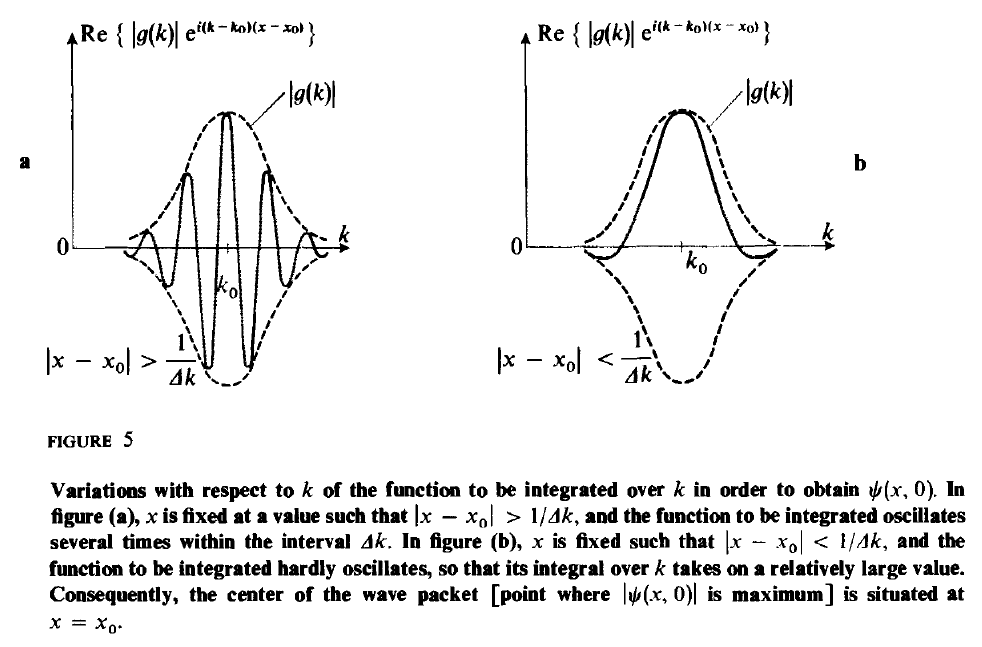
\includegraphics[scale=0.4]{Re(Psi) vs k.png}
\caption{\label{Re(Psi) vs k.png}}
\end{figure}
The position $x_M(0)$ of the center of the wave packet is:
$$
x_M(0)=x_0=-[\mathrm{d} \alpha / \mathrm{d} k]_{k=k_0}
$$
This result can be obtained by imposing the Stationary phase condition that the derivative with respect to $k$ of the phase is zero for $k=k_0$. In the particular case we are studying, the phase of the wave corresponding to $k$ is $k x+\alpha(k)$. Therefore, $x_M(0)$ is that value of $x$ for which the derivative $x+\mathrm{d} \alpha / \mathrm{d} k$ is zero at $k=k_0$. This means $k$ dependent phases vary slightly with $k$ around $k=k_0$. When $x$ moves away from the value $x_0,|\psi(x, 0)|$ decreases. This decrease becomes appreciable if $\mathrm{e}^{i\left(k-k_0\right)\left(x-x_0\right)}$ oscillates approximately once when $k$ traverses the domain $\Delta k$, that is, when:
$\Delta k .\left(x-x_0\right) \simeq 1$
If $\Delta x$ is the approximate  half width of the wave packet, we therefore have :
\begin{equation}
\Delta k \cdot \Delta x \gtrsim\frac{1}{2} 
\end{equation}
We are thus brought back to a classical relation between the widths of two functions which are Fourier transforms of each other. The important fact is that the product $\Delta x. \Delta k$ has a lower bound; the exact value of this bound depends on the precise definition of the widths $\Delta x$ and $\Delta k$.

A wave packet such as this represents the state of a particle whose probability of presence, at the time $t=0$, is practically zero outside an interval of approximate half width $\Delta x$ centered at the value $x_0$.\\
Comments:\\
It is assumed that $|\psi(x, 0)|$ has a single maximum as it is a  continuous superposition of infinitely many waves in a given interval of x. 
\subsubsection{Position and Momentum uncertainty principle}
In quantum mechanics, inequality (Eq 13) has significant physical consequences. Consider for simplicity, with the framework of a one-dimensional model
$\mathrm{e}^{i\left(k_0 x-\omega_0 t\right)}$. \\
This corresponds to a constant probability density for the particle's presence along the $x$ axis for all values. This result can be roughly expressed by saying that the corresponding value of $\Delta x$ is infinite. On the other hand, only one angular frequency $\omega_0$ and one wave vector $k_0$ are involved. According to the de Broglie relations, this means that the energy and momentum of the particle are well-defined: $E=\hbar \omega_0$ and $p=\hbar k_0$. Thus for such a plane wave $g(k)$ is a " delta function " :
$$
g(k)=\delta\left(k-k_0\right)
$$
The corresponding value of $\Delta k$ is then zero.
This property can also be interpreted in the following manner, using the principle of spectral decomposition. To say that a particle, described at $t=0$ by the wave function $\psi(x, 0)=A \mathrm{e}^{i k x}$, has a well-determined momentum, is to say that a measurement of the momentum at this time will definitely yield $p=\hbar k$. From this we deduce that $\mathrm{e}^{i k x}$ characterizes the eigenstate corresponding to $p=\hbar k$. Since there exists a plane wave for every real value of $k$, the eigenvalues which one can expect to find in a measurement of the momentum on an arbitrary state include all real values. In this case, there is no quantization of the possible results: as in classical mechanics, all values of the momentum are allowed.
Now consider the formula in the free particle wave packet. In this formula, $\psi(x, 0)$ appears as a linear superposition of the momentum eigenfunctions in which the coefficient of $\mathrm{e}^{i k x}$ is $g(k)$. We are thus led to interpret $|g(k)|^2$ (to within a constant factor) as the probability of finding $p=\hbar k$ if one measures, at $t=0$, the momentum of a particle whose state is described by $\psi(x, 0)$. In reality, the possible values of $p$, like those of $x$, form a continuous set, and $|g(k)|^2$ is proportional to a probability density: the probability $\overline{\mathrm{d} \mathscr{P}}(k)$ of obtaining a value between $\hbar k$ and $\hbar(k+\mathrm{d} k)$ is, to within a constant factor, $|g(k)|^2 \mathrm{~d} k$. More precisely, if we rewrite the formula in the free particle wave packet  in the form:
$$
\psi(x, 0)=\frac{1}{\sqrt{2 \pi \hbar}} \int \bar{\psi}(p) \mathrm{e}^{i p x / \hbar} \mathrm{d} p
$$
we know that $\bar{\psi}(p)$ and $\psi(x, 0)$ satisfy the Bessel-Parseval relation:
$$
\int_{-\infty}^{+\infty}|\psi(x, 0)|^2 \mathrm{~d} x=\int_{-\infty}^{+\infty}|\bar{\psi}(p)|^2 \mathrm{~d} p
$$
If the common value of these integrals is $C, \mathrm{~d} \mathscr{P}(x)=\frac{1}{C}|\psi(x, 0)|^2 \mathrm{~d} x$ is the probability of the particle being found, at $t=0$, between $x$ and $x+\mathrm{d} x$. In the same way:
$$
\overline{\mathrm{d} \mathscr{P}}(p)=\frac{1}{C}|\bar{\psi}(p)|^2 \mathrm{~d} p
$$
is the probability that the measurement of the momentum will yield a result included between $p$ and $p+\mathrm{d} p$ [The above relation ensures that the total probability of finding any value is indeed equal to 1].
Now let us go back to the inequality (Eq 13). We can write it as :
\begin{equation}
\Delta x . \Delta p \gtrsim \frac{\hbar} {2}
\end{equation}
$(\Delta p=\hbar \Delta k$ is the width of the curve representing $|\overline{\psi}(p)|)$. Consider a particle whose state is defined by the wave function at t=0. We know that its position probability at $t=0$, is appreciable only within a region of width $\Delta x$ about $x_0$ : its position is known within an uncertainty $\Delta x$. If one measures the momentum of this particle at the same time, one will find a value between $p_0+\frac{\Delta p}{2}$ and $p_0-\frac{\Delta p}{2}$, since $|\bar{\psi}(p)|^2$ is practically zero outside this interval : the uncertainty in the momentum is therefore $\Delta p$. The interpretation of relation (Eq 14) is then the following : it is impossible to define at a given time both the position of the particle and its momentum to an arbitrary degree of accuracy. When the lower limit imposed by (Eq 14) is reached, increasing the accuracy in the position (decreasing $\Delta x$ ) implies that the accuracy in the momentum diminishes ( $\Delta p$ increases), and vice versa. This relation is called the Heisenberg uncertainty relation.

We know of nothing like this in classical mechanics. The limitation (Eq 14) arises from the fact that $h$ is not zero. It is the very small value of $h$ on the macroscopic scale which renders this limitation negligible in classical mechanics.
\section{\label{sec:citeref}Citations and References}
\begin{enumerate}
\item Cohen Tannoudje-Quantum Mechanics
\item https://en.wikipedia.org/wiki/Bohr\_model
\end{enumerate}
\end{document}
%
% ****** End of file apssamp.tex ******
